% AUTORIGHTS
% Copyright (C) 2007 Princeton University
%       
% This file is part of Ferret Toolkit.
% 
% Ferret Toolkit is free software; you can redistribute it and/or modify
% it under the terms of the GNU General Public License as published by
% the Free Software Foundation; either version 2, or (at your option)
% any later version.
% 
% This program is distributed in the hope that it will be useful,
% but WITHOUT ANY WARRANTY; without even the implied warranty of
% MERCHANTABILITY or FITNESS FOR A PARTICULAR PURPOSE.  See the
% GNU General Public License for more details.
% 
% You should have received a copy of the GNU General Public License
% along with this program; if not, write to the Free Software Foundation,
% Inc., 51 Franklin Street, Fifth Floor, Boston, MA 02110-1301, USA.
\documentclass[]{article}

%\usepackage{code} 
\usepackage{epsfig}
\usepackage{verbatim} 

\paperwidth=8.5in
\paperheight=11in
\pdfpagewidth=\paperwidth
\pdfpageheight=\paperheight

\evensidemargin .05in  
\oddsidemargin .05in 
\setlength\topmargin{0.0 in}
\setlength\textheight{9.25in} \setlength\textwidth{6.25in} 
\setlength\columnsep{0.25in}  \newlength\titlebox  
\setlength\titlebox{2.0in} 
%\setlength\titlebox{2.375in} 
\setlength\headheight{0pt}   \setlength\headsep{0pt} 
%\setlength\footheight{0pt}   
\setlength\footskip{0pt} 

\begin{document}

\title{CASS (Content-Aware Similarity Search) Toolkit System Specifications}

\maketitle

% AUTORIGHTS
% Copyright (C) 2007 Princeton University
%       
% This file is part of Ferret Toolkit.
% 
% Ferret Toolkit is free software; you can redistribute it and/or modify
% it under the terms of the GNU General Public License as published by
% the Free Software Foundation; either version 2, or (at your option)
% any later version.
% 
% This program is distributed in the hope that it will be useful,
% but WITHOUT ANY WARRANTY; without even the implied warranty of
% MERCHANTABILITY or FITNESS FOR A PARTICULAR PURPOSE.  See the
% GNU General Public License for more details.
% 
% You should have received a copy of the GNU General Public License
% along with this program; if not, write to the Free Software Foundation,
% Inc., 51 Franklin Street, Fifth Floor, Boston, MA 02110-1301, USA.
\section {Toolkit Overview}

Figure \ref{fig:arch} shows the general architecture of the CASS toolkit.
For the first release, we are going to release a library (consists of
indexing modules, cass\_table modules, distance\_function modules
 and storage layer) as well
as a reference implementation which can be used to do content-aware
similarity search.

\begin{figure}[ht!]
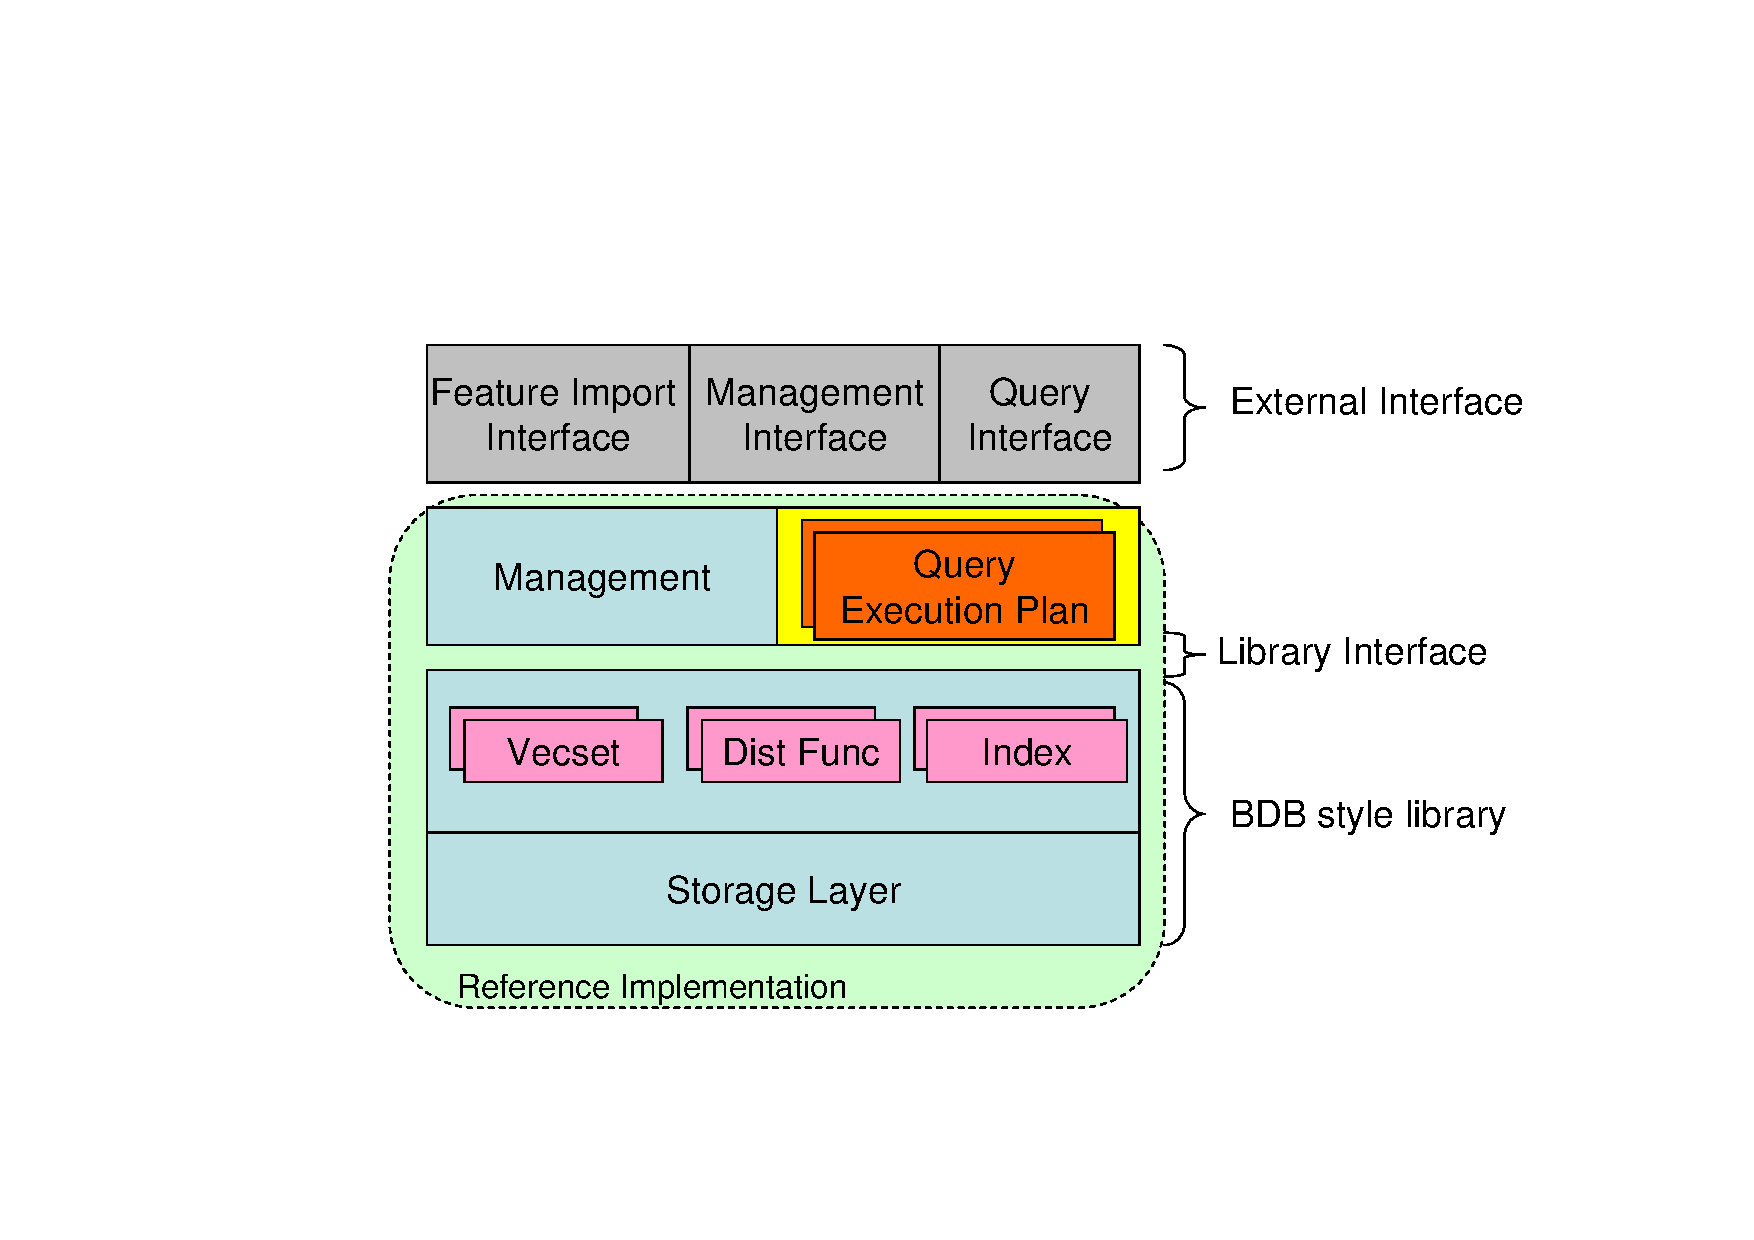
\includegraphics[clip=true,trim=1in 0.6in 0.1in 1.7in, width=0.8\textwidth]{cass_arch}
\caption{CASS Toolkit architecture}
\label{fig:arch}
\end{figure}

The following modules are part of the reference system for the
content-aware similarity search.
\begin{itemize}
\item Storage layer: Provides persistent storage for the system. It
  will support consistency via explicit checkpointing from
  application level. 
\item CASS\_table: They are DB table-like containers which store
  collection of cass\_vecsets which are feature representation of data\_objs.
\item Index: They are DB index like containers which store the index
  for cass\_table. Of note, they could index on cass\_vecset or
  cass\_vec.
\item Management: This is internal management module to manage
  index, cass\_tables, their associations and their placement
  (in-memory or not, where on disk)
\item Query Execution Plan: They are different ways of answering the
  query using different method to combine indexes and
  cass\_tables.
\end{itemize}

The following modules are external interfaces to the CASS system:
\begin{itemize}
\item Feature import interface: To import feature data into the system. 
\item Management interface: To manage and customize the CASS system.
\item Query interface: To satisfy end users' similarity search query.
\end{itemize}





% AUTORIGHTS
% Copyright (C) 2007 Princeton University
%       
% This file is part of Ferret Toolkit.
% 
% Ferret Toolkit is free software; you can redistribute it and/or modify
% it under the terms of the GNU General Public License as published by
% the Free Software Foundation; either version 2, or (at your option)
% any later version.
% 
% This program is distributed in the hope that it will be useful,
% but WITHOUT ANY WARRANTY; without even the implied warranty of
% MERCHANTABILITY or FITNESS FOR A PARTICULAR PURPOSE.  See the
% GNU General Public License for more details.
% 
% You should have received a copy of the GNU General Public License
% along with this program; if not, write to the Free Software Foundation,
% Inc., 51 Franklin Street, Fifth Floor, Boston, MA 02110-1301, USA.
\section{CASS Vecset}

We have three levels of feature related data structures in the system:
\begin{itemize}
\item cass\_vec: This is a single fix-sized feature vector. It could
  be a fix-sized array of floating point number, or a fix-sized L1
  sketch, or other compact feature representations. Eg: a 64 dimension
  color histogram is a cass\_vec.
\item cass\_vecset: This is individual cass\_vecset, which can be made up
  with a set of cass\_vecs. Eg: An image (represented here as a
  cass\_vecset) can contain a set of regions  where each region is
  represented by a cass\_vec.
\item cass\_table: This is a collection of cass\_vecsets. Eg:
  A collection of images used in content based similarity search
  corresponds to cass\_table.
\end{itemize}

To create correspondence of cass\_vecset with external world, we also
keep the mapping between cass\_vecset\_id and external data\_obj\_name
where data\_obj\_name is provided when the data are imported into the system.

Since we would like to allow import cass\_vecsets continuously, we would
allow the cass\_table to be present in memory when we grow the on-disk 
cass\_table. We would also try not to require restarting the whole
process after import a batch of vecsets.

\subsection{CASS Vector Related Data Structure}
\begin{verbatim}
typedef struct _cass_vecset_cfg_t {
    char *vecset_name;  // vecset_config can be shared between
                        // different datasets with same feature(eg: color hist)
    enum cass_vecset_type_t vecset_type; // TBD
    enum cass_vec_type_t cass_vec_type; // float_array, bitvec, vec_quant, etc.
    uint32_t cass_vec_size;  // number of bytes
    cass_vecset_flag_t flag;  // one flag: data_obj_name can be used
                                //           as vecset_id.
} cass_vecset_cfg_t; // one per vecset type

typedef cass_vecset_id_t uint32_t;

typedef struct _cass_table_t {
    cass_env_t *env;    // The containing cass_env.
    char *table_name;   // Name of the table, (when create/drop, use name)
    cass_vecset_cfg_t *cfg;
    cass_map_t *map;
    uint32_t *num_index;
    cass_idx_t *idxes;      // the set of indexes for this collection.
    bool vecsets_in_memory;  // Whether vecsets are in memory.
    cass_vecset_id_t num_vecsets;
    cass_vecset_t *vecsets; // If in memory: array of vecset indexed by
                              vecset_id, (size: num_vecsets)
    data_log_t *datalog;   // on disk storage.
} cass_table_t;

typedef struct _cass_vecset_t {
    uint32_t num_regions;
    cass_vec_t *cass_vecs;  // Array of cass_vec (size: num_regions)
} cass_vecset_t;    // continuously allocated indexed by vecset_id.

typedef struct _cass_vec_t {
    float_array | L1_sketch | multires_sketch | other;
    float weight;
    cass_vecset_id_t vecset_parent;  // vecset containing this cass_vec.
} cass_vec_t;

typedef struct _cass_map_t {
    char *dataset_name;   // same dataset can have multiple features.
    int num_tables;  // # of associated cass_tables.
    cass_table_t *tables; // tables that uses the map. 
    char **data_obj_name; // map: vecset_id => data_obj_name;
    hash_table data_obj_name => vecset_id.  // map: data_obj_name =>
                   // vecset_id (maybe not needed if user is required
		   // to provide vecset in the query.)
    data_log_t *data_log;  // note, if we separate map from the
                           // cass_table, it need its own storage.
} cass_map_t;

typdef struct _cass_qry_filterset_t {
    uint32_t num_ids;
    bool flag;  // Whether data_obj_names or ids are used.
    union {
        char **data_obj_names; 
	cass_vecset_id_t *ids;
    }
} cass_qry_filterset_t;  // Used to provide interface for external DB.

typedef struct _cass_qry_param_t {
    uint32_t topk;
    float range;
    char *extra_params;  // note: we can use more efficient repre if needed.
    cass_qry_filterset_t *filterset; // NULL means no filter.
} cass_qry_param_t;

typedef struct _cass_qry_result_t {
    uint32_t flag;  // eg: CASS_USERMEMORY
    cass_vecset_id_t num_results;
    cass_vec_t **vecs;   // array of pointers to vecs
} cass_qry_result_t;

enum {
        CASS_MALLOC       = 1<<0,
        CASS_REALLOC      = 1<<1,
        CASS_USERMEM      = 1<<2,
};

typedef struct _cass_datum_t {
        uchar   *data;
        u32int  size;
        u32int  ulen;
        u32int  flags;
} cass_datum_t;

\end{verbatim}

\subsection {Functions}
Interfaces to handle the cass\_tables:

\begin{verbatim}
cass_table_t *cass_table_create(cass_env_t *env,  // See management section
                                char *table_name,
                                cass_vecset_cfg_t *cfg, 
                                cass_map_t *map,
				data_log_t *datalog);
int cass_table_import_data(cass_table_t *table, char *fname); 
int cass_table_insert(cass_table_t *table,
                      cass_vecset_t *vecset);
int cass_table_checkpoint(cass_table_t *table, cass_datum_t **chkpnt_data);
                       // Initiate the checkpoint, upon success,
                       // return the chkpnt_data to store in the
                       // cass_env for checkpointing and future recovery.
int cass_table_restore_checkpoint(cass_table_t *table, cass_datum_t *chkpnt_data);
 
int cass_table_set_in_mem(cass_table_t *table, bool in_mem);
int cass_table_release_mem(cass_table_t *table);  // release in-mem data.
int cass_table_disk_to_mem(cass_table_t *table);  // bring data to in-mem.

int cass_table_associate_index(cass_table_t *table, 
                               cass_idx_t *idx);
int cass_table_disassociate_index(cass_table_t *table, 
                                  cass_idx_t *idx);
int cass_table_associate_table(cass_table_t *table, 
                               cass_table_t *tbl2);  // For auto sketching,etc.
int cass_table_disassociate_table(cass_table_t *table, 
                                  cass_table_t *tbl2);
int cass_table_destroy(cass_table_t *table);
                   // Destroy on-disk version as well.

// Note, if data is not in memory, this will trigger on-disk sequential scan.
// Need to add linear scan cursor interface.
int cass_table_query(cass_table_t *table, cass_vecset_t *qry_vecset, 
                     cass_qry_param_t *param, cass_qry_result_t *qry);
int cass_table_batch_query(cass_table_t *table, uint32_t count,
                           cass_vecset_t **qry_vecset,
                           cass_qry_param_t **params,
                           cass_qry_result_t **qries);
cass_datum_t *cass_table_meta_marshal(cass_table_t *table, cass_datum_t *data);
cass_table_t *cass_table_meta_unmarshal(cass_marshal_t *data); 
                   // marshal and unmarshal provide ways to
		   // save/restore the table/maps from/to env.

// Deal with cass_map_t.
cass_map_t *cass_map_create(cass_env_t *env, char *name, 
                                    data_log_t *datalog, bool flag);
     // flag says whether the dataobj name can be treated as id, 
     // then translation need no memory overhead.
int cass_map_associate_table(cass_map_t *map, cass_table_t *table);
int cass_map_disassociate_table(cass_map_t *map, cass_table_t *table);

int cass_map_insert(cass_map_t *map, cass_vecset_id_t *id,
                    char *dataobj_name); // Will return the id assigned.
int cass_map_disk_to_mem(cass_map_t *map, data_log_t *datalog);
cass_datum_t *cass_map_meta_marshal(cass_map_t *map, cass_datum_t *data);
cass_map_t *cass_map_meta_unmarshal(cass_marshal_t *data);

int cass_map_checkpoint(cass_map_t *map, cass_datum_t **chkpnt_data);
int cass_map_restore_checkpoint(cass_map_t *map, cass_datum_t *chkpnt_data);
\end{verbatim}


% AUTORIGHTS
% Copyright (C) 2007 Princeton University
%       
% This file is part of Ferret Toolkit.
% 
% Ferret Toolkit is free software; you can redistribute it and/or modify
% it under the terms of the GNU General Public License as published by
% the Free Software Foundation; either version 2, or (at your option)
% any later version.
% 
% This program is distributed in the hope that it will be useful,
% but WITHOUT ANY WARRANTY; without even the implied warranty of
% MERCHANTABILITY or FITNESS FOR A PARTICULAR PURPOSE.  See the
% GNU General Public License for more details.
% 
% You should have received a copy of the GNU General Public License
% along with this program; if not, write to the Free Software Foundation,
% Inc., 51 Franklin Street, Fifth Floor, Boston, MA 02110-1301, USA.
\section{Distance Functions}
New distance functions can be added by toolkit user. Also the
customized distance function (eg: L2 distance using only certain
dimensions from the cass\_vec) can be generated on the fly to satisfy
customized queries.

\subsection{CASS Distance Functions}
\begin{verbatim}
enum cass_vecset_type_t {any_vecset, single_cass_vec, set_of_cass_vecs,
  ...};
enum cass_cass_vec_type_t {any_cass_vec, float_array, L1_sketch,
  multires_sketch, ...};
enum cass_vecset_dist_measure_t {any_vecset_dist, emd,
  one_to_one_best_match, ...};
enum cass_cass_vec_distance_measure_t {any_cass_vec_dist, L1, L2, ...};

float (*cass_cass_vec_dist_func)(cass_cass_vec_t *f1, cass_cass_vec_t *f2);
float (*cass_vecset_dist_func)(cass_vecset_t *f1, cass_vecset_t *f2);

\end{verbatim}



% AUTORIGHTS
% Copyright (C) 2007 Princeton University
%       
% This file is part of Ferret Toolkit.
% 
% Ferret Toolkit is free software; you can redistribute it and/or modify
% it under the terms of the GNU General Public License as published by
% the Free Software Foundation; either version 2, or (at your option)
% any later version.
% 
% This program is distributed in the hope that it will be useful,
% but WITHOUT ANY WARRANTY; without even the implied warranty of
% MERCHANTABILITY or FITNESS FOR A PARTICULAR PURPOSE.  See the
% GNU General Public License for more details.
% 
% You should have received a copy of the GNU General Public License
% along with this program; if not, write to the Free Software Foundation,
% Inc., 51 Franklin Street, Fifth Floor, Boston, MA 02110-1301, USA.
\section{Index}

The system allows multiple kinds of indexing schemes to be
registered, eg: LSH, cover tree index, etc.

Cass\_table and index has one-to-many relationship:
one cass\_table can be associated with multiple indexes, while
any one index can only be associated with one cass\_table.

\begin{verbatim}
typedef _cass_idx_t {
    char *idx_name;
    cass_table_t *table;
    char *parameters;  // a copy of input paramters.
    int private_data_size;
    void *private_data;  // private data to store index-specific info.
} cass_idx_t;

char *cass_idx_estimate_paramters(cass_table_t *table);
cass_idx_t *cass_idx_create(cass_env_t *env, 
                            cass_table_t *table, char *parameters);
int cass_idx_insert(cass_idx_t *idx, cass_table_t *table, 
                    cass_vecset_t *vecset);
int cass_idx_batch_insert(cass_idx_t *idx, cass_table_t *table, 
                          cass_vecset_range_t range);  // not useful?
int cass_idx_query(cass_idx_t *idx, cass_vecset_t *qry_vecset, 
                   cass_qry_param_t *param, cass_qry_result_t *qry);
int cass_idx_batch_query(cass_idx_t *idx, uint32_t count,
                         cass_vecset_t **qry_vecset,
			 cass_qry_param_t **params,
			 cass_qry_result_t **qries);
int cass_idx_release_mem(cass_idx_t *idx);  // destroy in-mem index.
int cass_idx_checkpoint(cass_idx_t *idx, char *fname);
int cass_idx_from_disk(cass_idx_t *idx, char *fname); // idx was
                            // created by the management env.
int cass_idx_destroy(cass_env_t *env, cass_idx_t *idx);  // destroy on-disk index as well.

typdef struct _cass_idx_operations_t { 
    cass_idx_estimate_parameters,  // a set of function pointers.
    cass_idx_create,
    cass_idx_insert,
    cass_idx_query,
    cass_idx_release_mem,
    cass_idx_to_disk,
    cass_idx_from_disk,
    cass_idx_destroy,
    ...
} cass_idx_operations_t;

int cass_idx_register(char *idx_name, cass_idx_operations_t *idx_ops, 
                      enum cass_vecset_type_t vecset_type, 
		      enum cass_vec_type_t vec_type, 
		      enum cass_vecset_dist_measure_t dist_vecset,
		      enum cass_vec_distance_measure_t dist_vec,
		      ); 
    // Register idx_name, tell system what vecset_type, 
    // vec_type, dist_vecset, dist_vec it supports.
\end{verbatim}


% AUTORIGHTS
% Copyright (C) 2007 Princeton University
%       
% This file is part of Ferret Toolkit.
% 
% Ferret Toolkit is free software; you can redistribute it and/or modify
% it under the terms of the GNU General Public License as published by
% the Free Software Foundation; either version 2, or (at your option)
% any later version.
% 
% This program is distributed in the hope that it will be useful,
% but WITHOUT ANY WARRANTY; without even the implied warranty of
% MERCHANTABILITY or FITNESS FOR A PARTICULAR PURPOSE.  See the
% GNU General Public License for more details.
% 
% You should have received a copy of the GNU General Public License
% along with this program; if not, write to the Free Software Foundation,
% Inc., 51 Franklin Street, Fifth Floor, Boston, MA 02110-1301, USA.
\section {Storage Interface}
We provide a storage interface (datalog) which support append-only/read many
operations. The main user of the storage interface is the cass\_table
and cass\_map, where the items are appended to the storage in a
sequential order. We will also need to have checkpointing and
recovery capability. Note: The checkpoint/recovery information are
stored in the cass\_env rather than the datalog. 

\subsection {Checkpointing}
The checkpointing is done in the following manner: we would only support
checkpointing the full system. The checkpoint is done whenever the
system need to do so. (For the current sample application
implementation, we will checkpoint the system after every successful
import of feature file. So when the end user issued an import command,
the system will not return until the import and checkpointing is
successful. This way, the user will know easily where to restart if
the import failed.)

When the checkpointing is needed, the management code will freeze the
whole system and start checkpointing process. It will sync all
cass\_tables, cass\_maps to datalog and record the current maxlsn and
etc; it will save all the indexes to disk\_locx and 
finally it will save the management information to disk\_locx. The next
checkpoint will checkpoint all the cass\_tables, cass\_map, save
the indexes and management information to disk\_locy. By alternate the
disk\_locx and disk\_locy, we can always pick up the latest clean copy
and restore the full system to that stage. 

After all data are checkpointed (synced to disk), the cass\_env is
saved to a temporary file and ``atomically'' switched to a statically
defined file name called ``cass\_env.dat'' using rename system
call. This way the cass\_env.dat is always pointing to the latest
sucessful checkpoint. Upon system startup, we will check the
cass\_env, and restore the system to the consistent state.

\subsection {Storage API}
\begin{verbatim}
/*
 * All log records must be less than DataLogItemMax in size.
 *
 * All functions returning an int return 0 on success and -1 on
 failure.
 *
 * DataLogclose closes at log handle.
 * DataLogtruncate truncates the log to the specified LSN.
 * DataLogappend appends a cass_datum_t to the log and sets the new LSN.
 * DataLogmaxlsn returns the current maximum LSN.
 *
 * Mkdatalogiter creates a new log iterator; datalogiterclose closes
 it.
 * Datalogitersetlsn positions a log iterator at the specified LSN.
 * Datalogiternext returns the next log record and associated LSN.
 */
enum {
        DataLogVersion  = 1,
        DataLogItemMax  = 1<<22,
};

DataLog         *datalogopen(int omode, char *fname, int cr, 
                  void (*panic)(char*, ...), uint64_t lsn, uint64_t offset);
int             datalogclose(DataLog*);
int             datalogsync(DataLog*);  // Sync datalog to disk.
int             datalogtruncate(DataLog*, uint64_t offset);
int             datalogappend(DataLog*, cass_datum_t* data);
int             datalogmaxlsn(DataLog*, uint64_t* lsn, uint64_t* offset);
                  // Return current LSN and offset.

DataLogIter     *mkdatalogiter(DataLog*);
void            datalogiterclose(DataLogIter*);
//int           datalogitersetlsn(DataLogIter*, uint64_t); // Not supported.
int             datalogiternext(DataLogIter*, uint64_t*, cass_datum_t*);
\end{verbatim}



% AUTORIGHTS
% Copyright (C) 2007 Princeton University
%       
% This file is part of Ferret Toolkit.
% 
% Ferret Toolkit is free software; you can redistribute it and/or modify
% it under the terms of the GNU General Public License as published by
% the Free Software Foundation; either version 2, or (at your option)
% any later version.
% 
% This program is distributed in the hope that it will be useful,
% but WITHOUT ANY WARRANTY; without even the implied warranty of
% MERCHANTABILITY or FITNESS FOR A PARTICULAR PURPOSE.  See the
% GNU General Public License for more details.
% 
% You should have received a copy of the GNU General Public License
% along with this program; if not, write to the Free Software Foundation,
% Inc., 51 Franklin Street, Fifth Floor, Boston, MA 02110-1301, USA.
\section{Management Module}
The management module provide a working environment for cass\_table,
cass\_index and cass\_distfunc. It respond to user request to
add/remove table, indices, etc. 

\subsection {Management related API}
\begin{verbatim}

typedef struct _cass_env_t {
    // Internal management data for controlling the whole system 
    // similar to DB_ENV in BDB.
    // Need to hold all the meta data about tables, maps, indexes as well
    // as their checkpoint informations.
    
} cass_env_t; 

int cass_env_create(cass_env_t **env, uint32_t flags);
int cass_env_open(cass_env_t *env, char *db_home, uint32_t flags); 
      // Automatically recover to a consistent stage in case of crash.
int cass_env_close(cass_env_t *env, uint32_t flags);
int cass_env_err(cass_env_t *env, int error, const char *fmt, ...);

int cass_env_checkpoint(cass_env_t *env);
int cass_env_restorelastcheckpoint(cass_env_t *env);

// Control the system via cass_table_create, cass_idx_create etc.
// For simplicity, we will assume that we can load the table&index
// control structure into memory as part of cass_env upon system
// startup. This will simplify the management and enable on-disk
// sequential scan if needed since we know about the table even when 
// the data is not in memory.

// Need to add details on how to do checkpointing and recovery.
// Need details on external config file, what the user interface will
// look like, etc.
\end{verbatim}


% AUTORIGHTS
% Copyright (C) 2007 Princeton University
%       
% This file is part of Ferret Toolkit.
% 
% Ferret Toolkit is free software; you can redistribute it and/or modify
% it under the terms of the GNU General Public License as published by
% the Free Software Foundation; either version 2, or (at your option)
% any later version.
% 
% This program is distributed in the hope that it will be useful,
% but WITHOUT ANY WARRANTY; without even the implied warranty of
% MERCHANTABILITY or FITNESS FOR A PARTICULAR PURPOSE.  See the
% GNU General Public License for more details.
% 
% You should have received a copy of the GNU General Public License
% along with this program; if not, write to the Free Software Foundation,
% Inc., 51 Franklin Street, Fifth Floor, Boston, MA 02110-1301, USA.
\section{Query Execution Plan}

\begin{itemize}
\item Interface to external database is achieved by using
cass\_qry\_filterset\_t within the cass\_qry\_param\_t.
\item To support multiple modality, we would expose functions to
  support AND, OR, VOTE methods to combine results from different
  query results.
\end{itemize}

\subsection {Multiple modality support}
\begin{verbatim}
typdef struct _cass_fusion_param_t {
    enum cass_fusion_method_t method;  // AND, OR, VOTE, Weighted_SUM, etc
    union {
        method_specific_data;
    }
} cass_fusion_param_t;

int cass_fusion(cass_env_t *env, 
                uint32_t num_qries,
                cass_vecset_t **qry_vecset, 
                cass_qry_param_t **param, 
                cass_fusion_param_t *fusion_param;
                cass_qry_result_t *qry);
// Need to add details on combining results, eg: index + rerank;
                filter + rerank (using sketch or ori_feat), etc.
\end{verbatim}




\end{document}

